\chapter{Klassenbeschreibung Userinterface}

In diesem Kaptiel werden konkrete Attribute und Funktionalitäten der Klassen der App vorgestellt.

\section{View}

\subsection{Toolbar und Appmenü}

Das Userinterface der App besteht aus einer einzigen Activity ("`MainActivity"'), aus der heraus verschiedene Fragments aufgerufen werden können. Zu jedem Fragment gehört ein ViewModel.
In der MainActivity ist eine Toolbar definiert. In dieser Toolbar ist das Appmenü enthalten. Das Appmenü ist ein eigenes Fragment. Es wird über den Menübutton, der in der Toolbar liegt, aufgerufen und bietet über Buttons Zugriff zu verschiedenen ausgewählten Fragments.
Diese Fragments sind:
\begin{itemize}[nosep]
	\item RecipeListFragment: in Abb. \ref{menu} dargestellt durch Button: "`Meine Rezepte"'
	\item ShoppigListDisplayFragment: in Abb \ref{menu} dargestellt durch Button: "`Einkaufsliste"'
	\item FavouriteFragment: in Abb \ref{menu} dargestellt durch Button: "`Admin"'
	\item LoginFragment: in Abb \ref{menu} dargestellt durch Button: "`Login"'
	\item AdminFragment: in Abb \ref{menu} dargestellt durch Button: "`Admin"'
	\item FriendlistFragment (wenn \textbf{W14} implementiert ist): in Abb \ref{menu} dargestellt durch Button: "`Freunde"'
	\item FriendGroupFragment (wenn \textbf{W14} implementiert ist): in Abb \ref{menu} dargestellt durch Button: "`Gruppen"'
	\item Feed Fragment (wenn \textbf{W15} implementiert ist): in Abb \ref{menu} dargestellt durch Button: "`Feed"'
\end{itemize}

Implementiert: \textbf{F19, F25, F71}

\begin{figure}[H]
	\centering
	\includegraphics[width=0.7\textwidth]{pics/ToolbarMenu.png}%
	\caption{Toolbar mit angezeigtem Appmenü}%
	\label{menu}%
\end{figure}

Im Folgenden werden die einzelnen Fragments mitsamt ihren Inhalten beschrieben.

%Fragments
\subsection{CreateRecipeFragment}

\begin{figure}[H]
	\centering
	\includegraphics[width=0.7\textwidth]{pics/createRecipeFragment.png}%
	\caption{CreateRecipeFragment}%
	\label{view}%
\end{figure}
Implementiert: \textbf{F1, F2, F3, F4, F5, F6, F7, F8, F9, F10, F11, F13, F14, F15, F16, F20, F26, F32, F28, F29, F30, F31, F74, F75}
\begin{itemize}[nosep]
	\item 	Rezepttitel-EditText: Hier kann der Nutzer einen Titel für sein Rezept eingeben 
	\item 	Zubereitungszeit-EditText: Die Zeit, die zur Vorbereitung benötigt wird.
	\item 	Backzeit-EditText: Die Zeit, die das Gericht gebacken warten muss.
	
	\item 	Tagfeld-TextView: Hier kann der Nutzer Tags für sein Rezept hinzufügen. 
	
	\item Portionen-TextView: Das Portionen Feld
	\item PortionenAnzahl-EditText: Die Anzahl an Portionen, die man bei der Zubereitung des Rezepts bekommt. 
	\item Zutatenfeld-EditText: Alle Zutaten, die man zur Zubereitung des Gerichts braucht. Das Eingabeformat ist für jede Zutat "Menge Einheit Zutat", damit der Konvertierungsschritt zu einem öffentlich einsehbarem Rezept reibungslos abläuft.
	\item 	Zubereitung-Textfeld: Hier kann der Nutzer mit Text beschreiben, wie man das Rezept schrittweise zubereitet. Damit der Nutzer Überschriften in seiner Beschreibung hervorzuheben kann, gibt es die Möglichkeit die hervorzuhebenden Zeichen innerhalb zweier *-Symbole zu schreiben, wodurch beim Konvertieren zu einem öffentlichen Rezept diese Zeichen geparsed werden. Um andere Rezepte in seinem Text zu verlinken, kann der Nutzer den HTTP-Link eines Rezepts einfügen, um auf dieses Rezept verweisen. Diesem Link kann er ein Wort zuordnen, was statt des Links angezeigt wird.
	
	\item 	öffentlich-Switch: Falls der Nutzer sein Rezept veröffentlichen will kann er dies über den Schieberegler. Ist ein Rezept schon öffentlich und der Nutzer will dieses wieder als privat deklarieren ist das auch über diesen Regler machbar.
	
	\item 	Speichern-Button: Der Nutzer kann hierüber das Rezept in seiner Rezeptliste speichern. Falls der öffentlich-Schieberegler aktiviert ist, erfolgt die eine Vollständigkeitskontrolle und die Konvertierung.
	\item Teilen-Button: Der Nutzer hat die Möglichkeit hierüber das Rezept in andere Applikationen zu exportieren.
	\item Teilen-Button: Über den Speicher Button kann man das Rezept an externe Applikationen exportieren.
\end{itemize}


\subsection{RecipeListFragment}
\begin{figure}[H]
	\centering
	\includegraphics[width=0.7\textwidth]{pics/recipelistFragment.png}%
	\caption{RecipeListFragment}%
	\label{view}%
\end{figure}

Implements: \textbf{F17, F76, F77}

\begin{itemize}[nosep]
	\item header-TextView: Meine Rezepte Überschrift.
	\item  Rezeptliste mit je:
	\subitem	- Bearbeiten-Button: Hierüber kann der Nutzer sein Rezept bearbeiten.
	\subitem	- Rezeptname-TextView: Anzeige des Rezeptnamens.
	\subitem	- Entfernen-Button: Hierüber kann das jeweilige Rezept gelöscht werden
	\item 	Neues Rezept Erstellen-Button: Hierüber kann der Nutzer ein neues Rezept erstellen 
\end{itemize}



\subsection{AddEditCommentFragment}
\begin{figure}[H]
	\centering
	\includegraphics[width=0.7\textwidth]{pics/addeditCommentFragment.png}%
	\caption{AddEditCommentFragment}%
	\label{view}%
\end{figure}
Implementiert: \textbf{F37, F90}
\begin{itemize}[nosep]
	\item header-TextView: Hier wird "Neuer Kommentar angezeigt"
	\item 	Eingabe-Textfeld: Hier kann der Nutzer ein Kommentar in texlicher Form schreiben.
	\item 	Kommentieren-Button: veröffentlicht den Kommentar damit dieses in dem "RecipeDisplayFragment" gesehen werden kann
\end{itemize}

\subsection{DisplaySearchListFragment}
\begin{figure}[H]
	\centering
	\includegraphics[width=0.7\textwidth]{pics/displaysearchlistFragment.png}%
	\caption{DisplaySearchListFragment}%
	\label{view}%
\end{figure}
Implementiert: \textbf{F53, F54, F55, F58, F88}
\begin{itemize}[nosep]
	\item 	Auswahlbox-Spinner: Der Nutzer hat die Auswahl zwischen absteigend und aufsteigend.
	\item 	Auswahlbox-Spinner: Der Nutzer hat die Auswahl zwischen verschiedenen Suchfiltern.
	\item 	Rezeptliste-ScrollView: Hier warten alle Suchergebnisse sortiert angezeigt. Der Nutzer kann die jeweiligen Rezepte auswählen, und wird dann auf das "RecipeDisplayFragment" weitergeleitet.
\end{itemize}

\subsection{UserSearchFragment}
\begin{figure}[H]
	\centering
	\includegraphics[width=0.7\textwidth]{pics/user_search_fragment.png}%
	\caption{UserSearchFragment}%
	\label{view}%
\end{figure}
Implementiert: \textbf{F48, F59, F60, F61, F62, F98}
\begin{itemize}[nosep]
	\item  header-TextView: "Suchergebnisse"
	\item 	ID-EditText: Hier kann die Nutzer-ID des gesuchten Nutzers eingetragen werden.
	\item Suchen-Button: Der Nutzer wählt den Suchen Button und bekommt eine Ergebnisliste von Nutzern angezeigt, die auf die eingetragene ID passen.
	\item Nutzerliste: Hier werden alle Suchergebnisse angezeigt.
	\item Abo-Button: Hierüber kann man einem Nutzer abonnieren.
\end{itemize}



\subsection{PublicRecipeSearchFragment}
\begin{figure}[H]
	\centering
	\includegraphics[width=0.7\textwidth]{pics/publicRecipeSearchFragment.png}%
	\caption{PublicRecipeSearchFragment}%
	\label{view}%
\end{figure}
Implementiert: \textbf{F51, F52, F56, F57}
\begin{itemize}[nosep]
\item	Titelsuche-Textfield: Der Nutzer kann hier einen Rezepttitel eingeben, nachdem gesucht werden soll
\item	Zutatenhinzufügen-Textfield \& Button: über das Textfeld kann der Nutzer eine Zutat eingeben und über den Button in eine Liste eintragen

\item	Zutatenliste-TextView: Hier werden alle eingegebenen Zutaten gespeichert, mit denen gesucht werden soll

\item Zeit-TextView: Zeit Anzeige
\item Zeitminuten-EditText: Minuten Eingabe
\item	Tag-suchen-Button: Hierüber kommt der Nutzer zur Suche mit Tags
\item Mindestbewertung: Textanzeige und Rating-Bar-Button
\item	Tag-Anzeige: Hier werden die Tags angezeigt, die zur Suche genutzt werden sollen 
\item	Suchen-Button: Wenn der Nutzer seine Suchoptionen eingegeben hat, kann er über den Button die Suche starten
\end{itemize}


\subsection{FeedFragment}
\begin{figure}[H]
	\centering
	\includegraphics[width=0.7\textwidth]{pics/feedFragment.png}%
	\caption{FeedFragment}%
	\label{view}%
\end{figure}
Implementiert: \textbf{F70, F72}
\begin{itemize}[nosep]
	\item header-TextView: "Feed" Anzeige
	\item	RezeptListe: Hier werden alle Rezepte des Feeds angezeigt und können vom Nutzer ausgewählt werden. Dann kommt der Nutzer auf das jeweilige "RecipeDisplayFragment".
\end{itemize}
Der Feed zeigt die aktuellsten Rezepte an, die veröffentlicht wurden. Bei jedem neuen Laden des Feeds wird die Ansicht aktualisiert.

\subsection{ProfileDisplayFragment}
\begin{figure}[H]
	\centering
	\includegraphics[width=0.7\textwidth]{pics/profilDistplayFragment.png}%
	\caption{ProfileDistplayFragment}%
	\label{view}%
\end{figure}
Implementiert: \textbf{F47, F63, F91}
\begin{itemize}[nosep]
	\item Namensfeld-TextView: Hier wird die Benutzer-ID angezeigt
	
	\item Folgen-Button:Hier kann man dem angezeigten Nutzer folgen.
	
	\item Beschreibung-TextView: Hier wird angezeigt, wie sich der Nutzer in ein paar wenigen Sätzen beschrieben hat. 
	
	\item Profilbild-ImageView: Der Benutzer kann ein Profilbild anzeigen lassen. Falls er dies nicht will, wird ein Standardbild angezeigt.
	
	\item Profilmelden-Button: falls ein Profil unangemessene Inhalte enthält, kann dieses hierdurch gemeldet werden, worauf es manuell von einem Admin geprüft wird.
	
	\item Freund+-Button: Nutzer können hierdurch anderen Nutzern eine Freundschaftsanfrage schicken
	
	\item Erstellte Rezepte-Liste: Hier werden alle öffentlich gestellten Rezepte des Nutzers angezeigt. Wenn man eins auswählt, kommt man direkt zum jeweiligen "RecipeDisplayFragment".
\end{itemize}

\subsection{ProfileEditFragment}
\begin{figure}[H]
	\centering
	\includegraphics[width=0.7\textwidth]{pics/profileEditragment.png}%
	\caption{ProfileEditFragment}%
	\label{view}%
\end{figure}
Implementiert: \textbf{F41, F43, F44, F45, F46, F42}
\begin{itemize}[nosep]
	\item BenutzerID-EditView: Hier kann die Benutzer-ID eingetragen werden
	\item Profilbild-ImagView: Hier kann der Nutzer ein Profilbild hochladen und ändern.
	\item Beschreibung-Textfield: Hier kann sich der Nutzer in ein paar Worten selbst beschreiben. Dies ist auch in der öffentlichen Ansicht des Nutzerprofils sichtbar.
	\item Login-Daten-Ändern-Button: Falls der Nutzer seine Anmelde-Daten ändern möchte, kann er dies mit diesem Button machen
	\item Speichern-Button: der Nutzer speichert über diesen Button die Änderungen für sein Profil.
	\item löschen-Button: Hierüber entfernt der angemeldete Nutzer sein Profil, wodurch alle seine Daten, bis auf die privaten Rezepte, gelöscht werden.
\end{itemize}
Auf diesem Fragment kann der Nutzer alle öffentlich angezeigten Informationen ändern. Will er seine Daten zum Einloggen ändern erreicht er dies über den Login Daten ändern Button.

\subsection{RegistrationFragment}
\begin{figure}[H]
	\centering
	\includegraphics[width=0.7\textwidth]{pics/registrationFragment.png}%
	\caption{RegistrationFragment}%
	\label{view}%
\end{figure}
Implementiert: \textbf{F38, F39}
\begin{itemize}[nosep]
	\item header-TextView:"Registrieren"-Kopfzeile
	\item Email-Adresse-Textfield: Hier kann der Nutzer seine Email Adresse angeben
	\item Passwort-EditText:Hier kann der Nutzer sein Passwort angeben
	\item Benutzer ID -EditText: Hier kann der Nutzer eine Wunsch ID eintragen. Macht er dies nicht wird bei der Registrierung automatisch eine erstellt. 
	\item Registrieren-Button: Wenn der Nutzer seine Daten eingetragen hat, kann er über diesen Button die Registrierung abschließen
\end{itemize}
Bei der Registrierung hat der Nutzer drei Eingabefelder gegeben. Die Pflichtfelder für eine erfolgreiche Registrierung sind die Email-Adresse und  Passwort. Gibt der Nutzer diese gar nicht oder fehlerhaft an, wird der Prozess nicht weitergeführt. Des Weiteren kann der Nutzer eine BenutzerID für sich festlegen. Die Benutzer-ID und das Passwort können im Nachhinein noch geändert werden und sind nicht permanent. Die Email hingegen ist ab der erfolgreichen Registrierung nicht mehr änderbar.

\subsection{ChangePasswordFragment}
\begin{figure}[H]
	\centering
	\includegraphics[width=0.7\textwidth]{pics/change_password_fragment.png}%
	\caption{ChangePasswordFragment}%
	\label{view}%
\end{figure}
Implementiert: \textbf{F40}
\begin{itemize}[nosep]
	\item Passwort-Textfield: Hier kann der angemeldete Nutzer sein neues Passwort eingeben.
	\item Passwort ändern - Button: Hierüber bestätigt der Nutzer sein neues Passwort
	
\end{itemize}
Da die Applikation die Account Funktionalität über Firebase verwaltet, werden die eingetragenen Daten direkt weitergegeben und so wenig wie möglich selbst gehalten. 


\subsection{LoginFragment}
\begin{figure}[H]
	\centering
	\includegraphics[width=0.7\textwidth]{pics/loginFragment.png}%
	\caption{LoginFragment}%
	\label{view}%
\end{figure}
Implementiert: \textbf{F50}
\begin{itemize}[nosep]
	\item Email-Textfield: Hier kannn der Nutzer seine Email angeben
	\item Passwort-Textfield:Hier kann der Nutzer sein Passwort angeben
	\item Login-Button: Wenn der Nutzer seine Daten eingetragen hat, kann er sich über diesen Button einloggen.
	\item Registrieren-Button: Falls der Nutzer noch kein Account hat, kann er auf den Registrieren Button klicken, um auf das RegistrationFragment geleitet zu werden.
\end{itemize}

\subsection{EditTagFragment}
\begin{figure}[H]
	\centering
	\includegraphics[width=0.7\textwidth]{pics/editTagFragment.png}%
	\caption{EditTagFragment}%
	\label{view}%
\end{figure}
Implementiert: \textbf{F73}
\begin{itemize}[nosep]
	\item Tag-Textfield: Hier kannn der Nutzer seine neuen Tags eingeben
	\item +-Button: Falls der Nutzer neue Eingabefelder braucht, kann er über den Button diese anfordern
	\item Speichern-Button: Wenn der Nutzer seine Tags eingetragen hat, kann er über den Speichern Button die Erstellung abschließen
\end{itemize}

\subsection{SearchWithTagsFragment}
\begin{figure}[H]
	\centering
	\includegraphics[width=0.7\textwidth]{pics/searchWithTagsFragment.png}%
	\caption{SearchWithTagsFragment}%
	\label{view}%
\end{figure}
\begin{itemize}[nosep]
	\item Tag-Auflistung: Hier werden alle vom User gesammelten Tags aufgelistet. Diese kann der Nutzer über eine Auswahlbox markieren.
	\item Fertig-Button: Wenn der Nutzer seine gewünschten Tags gesammelt hat, mit denen er suchen will, kann er über den Fertig-
	Button zurück zur Rezeptsuche gehen, wobei die Tags mitgenommen werden.

\end{itemize}

\subsection{AdminFragment}
\begin{figure}[H]
	\centering
	\includegraphics[width=0.7\textwidth]{pics/adminFragment.png}%
	\caption{AdminFragment}%
	\label{view}%
\end{figure}

\begin{itemize}[nosep]
	\item Nutzer-Auflistung: Hier sieht der Admin alle gemeldeten Nutzer. Er kann sich die Profile ansehen und einzelne nicht erlaubte Einträge (Bild, ID, Beschreibung) entfernen
	\item Rezept-Auflistung:Hier sieht der Admin eine Liste von allen gemeldeten Rezepten. er kann diese manuell überprüfen und direkt über den Button entfernen. 
	\item Gruppen-Auflistung: Hier sieht der Admin alle Gruppen, die gemeldet wurden. Falls ein Gruppenname nicht erlaubt ist, kann der Admin über den Button die Gruppe auflösen.
\end{itemize}
Der Admin hat über die Applikation die Möglichkeit Rezepte und Gruppen direkt zu entfernen. Falls ein Nutzer ein unpassenden Namen, Beschreibung, oder Bild hat muss sich der Admin dieses manuell ansehen und entscheiden, ob nur das jeweilige Feld aus der Datenbank austrägt, oder den Nutzer komplett entfernt.

\subsection{ShoppingListDisplayFragment}
\begin{figure}[H]
	\centering
	\includegraphics[width=0.7\textwidth]{pics/shoppingListdisplayFragment.png}%
	\caption{ShoppingListDisplayFragment}%
	\label{view}%
\end{figure}
Implementiert: \textbf{F21, F24}
\begin{itemize}[nosep]
	\item Zutaten-Auflistung: Hier werden alle Zutaten, die der Nutzer seiner Einkaufliste hinzugefügt an angezeigt. Diese kann er über eine Checkbox abhaken. 
	\item leeren-Button: Falls die Liste nicht mehr benötigt wird, kann der Nutzer diese über den Button leeren.
\end{itemize}

\subsection{FriendListFragment}
\begin{figure}[H]
	\centering
	
	\includegraphics[width=0.7\textwidth]{pics/friendListFragment.png}%
	\caption{FriendListFragment}%
	\label{view}%
\end{figure}
Implementiert: \textbf{F64, F65, F66, F92}
\begin{itemize}[nosep]
	\item Freundesauflistung:Hier werden alle schon bestätigten Freunde des Nutzers angezeigt. Wenn man eine Person anklickt, kommt man zur jeweiligen Profilansicht.  
	
	\item Freundschaftsanfragen:Hier werden alle Nutzer angezeigt, die eine Freundschaftsanfrage gesendet haben. Wenn man eine Person anklickt, kommt man zur jeweiligen Profilansicht. 
	\item Suchen-Button: Hierüber kommt man zu einer Ansicht, die eine Benutzersuche bereitstellt
	\item Entfernen-Button: Der Freund wird aus der Freundesliste entfernt
	\item Hinzufügen-Button: Der Freund wird der Freundesliste hinzugefügt
\end{itemize}

\subsection{GroupMemberListFragment}
\begin{figure}[H]
	\centering
	
	\includegraphics[width=0.7\textwidth]{pics/groupMemberListFragment.png}%
	\caption{GroupMemberListFragment}%
	\label{view}%
\end{figure}


\begin{itemize}[nosep]
	\item Gruppenname-TextView: Name Der Gruppe 
	\item Gruppenmitglieder-Auflistung:Hier werden alle Mitglieder der Gruppe aufgelistet. Wenn man sie auswählt, kommt man zur jeweiligen Profilansicht.
\end{itemize}


\subsection{CreateGroupFragment}
\begin{figure}[H]
	\centering
	\includegraphics[width=0.7\textwidth]{pics/createGroupFragment.png}%
	\caption{CreateGroupFragment}%
	\label{view}%
\end{figure}
Implementiert: \textbf{F67, F68, F93, F94}
Wir müssen auch sorgen, das im nachinein Mitglieder hinzugefügt werden können, dafür kann ja dieses Fragment recycled werden
\begin{itemize}[nosep]
	\item Gruppenname-TextView: Gruppenname wird angezeigt
	\item Freunde-Auflistung:Hier werden alle Freunde des Nutzers aufgelistet. Über die Checkbox auf der rechten Seite kann man einen Gruppe beim Erstellen der Gruppe hinzufügen. Drückt man auf einen Nutzer, kommt man nicht auf die jeweilige Profilseite.
\end{itemize}

\subsection{FriendGroupFragment}
\begin{figure}[H]
	\centering
	\includegraphics[width=0.7\textwidth]{pics/friendGroupFragment.png}%
	\caption{FriendGroupFragment}%
	\label{view}%
\end{figure}
Implementiert: \textbf{F68, F95}
\begin{itemize}[nosep]
	\item Gruppen-Auflistung: Hier werden alle Gruppen, in denen der Nutzer Mitglied ist, aufgelistet. 
	\item Löschen-Button
	\subitem - Falls er der Admin ist, wird die Gruppe komplett entfernt
	\subitem - Falls er nicht der Admin ist, entfernt er nur sich aus der Gruppe
	\item Gruppe-erstellen-Button: Hierüber kommt der Nutzer auf die Gruppe-Erstellen Ansicht.
\end{itemize}

\subsection{GroupFragment}
\begin{figure}[H]
	\centering
	\includegraphics[width=0.7\textwidth]{pics/groupFragment.png}%
	\caption{GroupFragment}%
	\label{view}%
\end{figure}
Implementiert: \textbf{F69}
\begin{itemize}[nosep]
	\item Gruppenname: Hier wird der Gruppenname angezeigt und wenn man darauf klickt, kommt man auf die Gruppenmitglieder Ansicht
	\item Rezept-Auflistung: Hier werden alle geteilten Rezepte aufgelistet. Wenn man diese anklickt, kommt man auf die Rezept bearbeiten Ansicht. Da man private Rezepte in Gruppen teilen kann, können diese unvollständig sein. Daher kann man diese nur in der bearbeiten Ansicht anschauen.
\end{itemize}

\subsection{RecipeDisplayFragment}
\begin{figure}[H]
	\centering
	\includegraphics[width=0.7\textwidth]{pics/recipeDisplayFragment.png}%
	\newline
    \includegraphics[width=0.7\textwidth]{pics/recipeDisplayFragmentzwei.png}%
	\caption{RecipeDisplayFragment}%
	\label{view}%
\end{figure}
Implementiert: \textbf{F18, F22, F23, F33, F34,F35, F36}
\begin{itemize}[nosep]
	\item Rezeptbild: Hier wird das Rezeptbild angezeigt
	\item Rezepttitel: Der Name des Rezepts
	\item Bewertungsfeld: Hier kann jeder angemeldete Nutzer eine Bewertung für das Rezept angeben
	\subitem Falls das Rezept schon vom Nutzer bewertet wurde, wird diese Bewertung angezeigt
	\item Zubereitungszeit: Hier steht die Zeit, die für die Zubereitung benötigt wird
	\item Backzeit: Hier steht die Zeit, die das Gericht gebacken werden muss
	\item Gesamtzeit: Diese ergibt aus der Zubereitungs- und der Backzeit
	\item Einkaufsliste-Button: Hierüber kann der Nutzer die Zutaten in seine Einkaufsliste eintragen. Daraufhin kommt er auch in die Einkaufslisten Ansicht
	\item skalieren-Button: Wenn der Nutzer eine neue Menge eingibt, werden die Portionen umgerechnet.
	\item Profilbild: Hier wird das Profilbild des Rezepterstellers angezeigt. Wenn man dieses anklickt, kommt man auf die Profilansicht des Erstellers.
	\item Hinzufügen-Button: Wenn man diesen anklickt, wird das Rezept in der Favoritenliste hinzugefügt
	\item Zutaten-Liste: Hier werden alle für das Rezept benötigten Zutaten aufgelistet
	\item Tag-Liste: Hier werden alle von dem Autor eingetragenen Tags angezeigt
	\item Beschreibung: Hier steht die Zubereitungsbeschreibung für das Rezept
	\item Kommentar schreiben - Button: Hier kann ein angemeldeter Nutzer ein Kommentar zu dem jeweiligen Rezept verfassen. Hierüber wird man auf das AddEditCommentFragment weitergeleitet. 
	Klick man auf ein Kommentar, das von einem selbst ist, wird man auf das AddEditCommentFragment weitergeleitet. 
	\item Kommentarliste: Hier werden alle zu dem Rezept schon verfassten Kommentare aufgelistet.
	\item Melden-Button: Hierüber kann das Rezept gemeldet werden. Daraufhin erscheint das Rezept in der Liste des Admins, der dieses dann manuell überprüfen kann. 
	
\end{itemize}

\subsection{FavouriteFragment}
\begin{figure}[H]
	\centering
	\includegraphics[width=0.7\textwidth]{pics/favouriteFragment.png}%
	\caption{FavouriteFragment}%
	\label{view}%
\end{figure}


\begin{itemize}[nosep]
	\item Rezeptliste: Hier werden alle favorisierten Rezepte angezeigt. Diese kann der Nutzer einzeln aus der Favoritenliste entfernen. Wenn auf ein Rezept geklickt wird, kommt man auf die jeweilige Rezeptansicht des Rezepts.
	\item entfernen-Button: Das Rezept wird gelöscht
\end{itemize}

%ViewModels
\newpage
\section{ViewModel}
Im Folgenden werden die den Fragments zugehörigen ViewModel-Klassen beschrieben.
Vorweg sei gesagt, dass alle ViewModels in der onCreate()-Methode der Main-Activity eingebunden werden müssen.
Jedes einzelne ViewModel wird außerdem in dem ihm zugehörigen Fragment instanziiert. Somit wird beim allerersten Aufruf des Fragments sein ViewModel erstellt, sodass dieses Daten für das Fragment bereitstellen kann.
Da Die Viewmodel an einigen Stellen einen redundanten Aufbau besitzen, werden die wichtigen Eigenheiten des ViewModels in der folgenden Beschreibung hervorgehoben. Ist ein Repository eingezeichnet, so sind die darin  beschriebenen Methoden aus Übersichtsgründen nur auf das jeweilige ViewModel abgestimmt. Im Entwurf wird es dennoch nur eine Klasse geben, das alle vorkommenden Methoden der ViewModel beinhaltet. Der Ablauf ist jeweils immer gleich, dass ein Fragment sein zugehöriges ViewModel erstellt, worüber der Zugriff auf das Repository stattfindet. Damit ist die Oberfläche der Applikation sauber von der Datenquelle getrennt. Die Relation zwischen dem jeweiligen ViewModel und dem Fragment ist über ein Oberserver Pattern beschrieben. Exemplarisch ist das im DisplaySearListViewModel näher erläutert. Dieses Obersever-Pattern soll für die weiteren ViewModel implizit angenommen werden, da es aus Redundanzgründen und der Übersichtlichkeit nicht modelliert wurde. Ähnlich redundant ist der Aufbau der Fragmente, der prinzipiell den Klassen entspricht, wie oben beschrieben  (Siehe Kapitel 5.1). Daher wurden die Fragmente nur skizzenhaft modelliert und nur eingefügt, wo es der Übersicht hilft.

\subsection{DisplaySearchListViewModel}
\begin{figure}[H]
	\centering
	\includegraphics[width=0.7\textwidth]{pics/viewModel/Display_Search_List_ViewModel.pdf}%
	\caption{DisplaySearchList}%
	\label{viewModel}%
\end{figure}

\begin{itemize}
	\item \textcolor{blue}{DisplaySearchListViewModel(title:String, ingredients:List<String>, rating:int, tags:List<String>, time:int)}\textcolor{cyan}{:constructor} Im Konstruktor werden alle Suchparameter übergeben \textbf{F53, F54, F56}
	
	\item \textcolor{blue}{sortRecipes()}\textcolor{cyan}{:void} Diese Methode sortiert die aufgelisteten Rezepte nach dem gewünschten Kriterium. Der Nutzer kann das Kriterium in einer Ausklappbaren Leisten im Fragment auswählen. Diese Kriterien beinhalten beispielsweise: Datum, Bewertung,... \textbf{F55, F58} 
	
	\item \textcolor{blue}{getRecipes()} \textcolor{cyan}{:List<PublicRecipe>} Diese Methode lädt die jeweiligen Rezepte, die auf die Eingaben des "PublicRecipeSearchFragment" passen, aus dem Repository.
\end{itemize}

\subsubsection{Observer Entwurfsmuster}
Observer
Durch den Observer ist es möglich eine saubere Kapselung der Schichten in nur eine Richtung zu halten. Die View Schicht kennt die ViewModel schicht, jedoch nicht andersherum. Um trotzdem aktuell zu bleiben, nutzt man das Oberserver Pattern. Die ViewModel Schicht hält die View Schicht nicht als Assoziation, sondern wird automatisch bei einer Änderung benachrichtigt, dass sich was geändert hat. Damit gehört es zu den Verhaltensmustern und dient der Weitergabe von Änderungen an einem Objekt an von diesem Objekt abhängige Strukturen.




\subsection{CreateRecipeViewModel}
\begin{figure}[H]
	\centering
	\includegraphics[width=0.7\textwidth]{pics/viewModel/Create_Recipe_ViewModel.pdf}%
	\caption{CreateRecipeViewModel}%
	\label{viewModel}%
\end{figure}

\begin{itemize}
	\item \textcolor{blue}{CreateRecipeViewModel(privateRec:PrivateRecipe)}\textcolor{cyan}{:constructor} Wenn ein bestehendes Rezept bearbeited werden soll, wird dieses im Konstruktor übergeben und sonst ein null Pointer \textbf{F15}

	\item \textcolor{blue}{addTags()}\textcolor{cyan}{:void} öffnet das  SearchWithTagsCreateRecipeFragment 
	
	\item \textcolor{blue}{setContent(title:String, preppingtime:Int, cookingtime:Int, servings,ingredients:List<String>, description:String, idPublic:String)}\textcolor{cyan}{:void} schreibt die bisher eingetragenen LiveData-Attribute (!=null) in das Rezept \textbf{F2, F3, F4, F5, F6, F7, F8, F9, F10}
	
	\item \textcolor{blue}{addToRepository(rec:PrivateRecipe}\textcolor{cyan}{:void} ruft erst setContent(...) auf und gibt dann das privateRecipe an das Repository zum Speichern in der SQLite DB
	
	\item \textcolor{blue}{parse(rec:PrivateRecipe)} \textcolor{cyan}{:PublicRecipe} wandelt das PrivateRecipe rec in ein PublicRecipe um. Dazu prüft die Methode alle Attribute des PrivateRecipe. Außerdem werden die HTTP-Links aus der Zubereitungsbeschreibung geprüft. Ist ein Link nicht gültig, wird der Nutzer mithilfe eines Alert-Dialogs gewarnt \textbf{F32}
	
	\item \textcolor{blue}{save()}\textcolor{cyan}{:void} unterscheidet, ob isPublic={true,false}.
	true: rufe parse() mit privateRec als Parameter auf 
	und schicke dann das Resultat ins Repository
	zum Speichern auf dem Server
	false: speichert Rezept nur lokal \textbf{F1, F11, F14}
	
	\item \textcolor{blue}{addToRepository(parse(privateRec))}\textcolor{cyan}{:void}
	false: rufe addToRepository(privateRecipe) auf und
	lasse somit das privateRec vom Repository in der 
	SQLite DB speichern. \textbf{F13, F16}
	
	
	
\end{itemize}


\subsection{RecipeListViewModel}
\begin{figure}[H]
	\centering
	\includegraphics[width=0.7\textwidth]{pics/viewModel/Recipe_List_ViewModel.pdf}%
	\caption{RecipeListViewModel}%
	\label{viewModel}%
\end{figure}
\begin{itemize}
	\item \textcolor{blue}{getPrivateRecipes()}\textcolor{cyan}{:List<PrivateRecipe>}
	alle privaten Rezepte werden geladen.
	\item  \textcolor{blue}{deletePrivateRecipe(id:String)}\textcolor{cyan}{:void}
	löscht ein privates Rezept. Falls dieses öffentlich ist, wird dieses auch vom Server entfernt \textbf{F17}
	\item \textcolor{blue}{editPrivateRecipe(recipe:PrivateRecipe)}\textcolor{cyan}{:void}Diese Methode löst einen Fragment wechsel aus, wobei das ausgewählte Rezept in das "CreateRecipeFragment" übergeben wird
	\item \textcolor{blue}{createnewRecipe()}\textcolor{cyan}{:void}
	Diese Methode löst einen Fragmentwechel aus, wobei auf das "CreateRecipeFragment" mit unausgefülltem Template gewechselt wird
\end{itemize}


\subsection{AddEditCommentViewModel}
\begin{figure}[H]
	\centering
	\includegraphics[width=0.7\textwidth]{pics/viewModel/AddEdit_Comment_ViewModel.pdf}%
	\caption{AddEditCommentViewModel}%
	\label{viewModel}%
\end{figure}
\begin{itemize}
	\item \textcolor{blue}{AddEditCommentViewModel(recipeId:int, commentId:int)} \textcolor{cyan}{:construct} Wenn ein Kommentar bearbeitet werden soll, wird die commentId hier übergeben
	
	\item \textcolor{blue}{addCommentToRecipe(...)} \textcolor{cyan}{:void}
	Ordnet dem Rezept über das Repository ein neues Kommentar hinzu, 
	falls die commentID noch nicht existiert. Falls die
	schon existiert, wird das bisherige ersetzt.
	
	\item \textcolor{blue}{loadComment(id:int)}\textcolor{cyan}{:Comment} 
	fragt über das Repository den Server an, ob ein Kommentar mit der 
	gegebenen ID existiert.Falls ja wird dieses zurückgegeben.
	
\end{itemize}
Der Nutzer ist hier, um ein Kommentar zu einem Rezept zu schreiben. Falls er ein schon bestehendes Kommentar ändern will, wird dieses schon in dem Textfeld angezeigt. Will der Nutzer ein neues Kommentar verfassen ist das Textfeld leer. Falls der Nutzer ein leeres Textfeld speichern will, kehrt der Nutzer auf das "RecipeDisplayFragment" zurück, ohne dass ein Kommentar hinzugefügt wird. 





\subsection{UserSearchViewModel}
\begin{figure}[H]
	\centering
	\includegraphics[width=0.7\textwidth]{pics/viewModel/User_Search_ViewModel.pdf}%
	\caption{UserSearchViewModel}%
	\label{viewModel}%
\end{figure}
\begin{itemize}
	\item \textcolor{blue}{followUser(userID:String)}\textcolor{cyan}{:void}  fügt den übergebenen User in die Abonnementliste des Senders ein. \textbf{F48}
	
	\item \textcolor{blue}{getUsers(userID:String)}\textcolor{cyan}{:List<User>} gibt die User, deren ID mit userID beginnt, zurück. \textbf{F59, F60, F61}
\end{itemize}
Jeder Nutzer kann über die Sucheingabe die Benutzer-ID eines registrierten Nutzers eingeben. Klickt er dann auf "`suchen"', so werden in einer Liste alle passenden Ergebnisse angezeigt. Die Benutzer-ID muss eindeutig sein. Trotzdem ergibt es Sinn, auch verschiedene Suchergebnisse anzuzeigen, da der Suchende eventuell nur ein Präfix der eigentlichen ID kennt, oder eingegeben hat. Demnach sollen alle Nutzer angezeigt werden, die auch diesen Präfix beinhalten. 
Im Pflichtenheft wurde beschrieben, dass die Benutzersuche durch mehrere Suchfilter eingeschränkt werden kann. Da die Architektur der Applikation in ihrer Grundfunktion jedoch nicht darauf ausgelegt ist, weil vorerst die ID der primäre eindeutige Bezeichner für einen angemeldeten Nutzer ist, wird diese Funktion nicht implementiert.

\subsection{PublicRecipeSearchViewModel}
\begin{figure}[H]
	\centering
	\includegraphics[width=0.7\textwidth]{pics/viewModel/Public_Recipe_Search_VieModel.pdf}%
	\caption{PublicRecipeSearchViewModel}%
	\label{viewModel}%
\end{figure}
\begin{itemize}
	\item  \textcolor{blue}{addIngredientToList()}\textcolor{cyan}{:void}
	Fügt der Suchliste Zutaten hinzu.
	\item  \textcolor{blue}{addTags()}\textcolor{cyan}{:void} öffnet das SearchWithTagsFragment
	\item \textcolor{blue}{search(title:String, ingredients:List<String>, rating:int, tags:List<String>, time:int)} \textcolor{cyan}{:void} Diese Methode übergibt dem DisplaySearchListFragment die Suchparameter \textbf{F51, F52}
	
\end{itemize}
Die Spezifikation, dass Zubereitungsbeschreibung ein Suchfilter darstellt, wurde aus verschiedenen Gründen nicht in den Entwurf übernommen. Die Suchkernfunktionalität der Applikation liegt auf der Suche mit Titel, Zutaten und Tags. Die Beschreibung ist jedoch mehr für den Zubereitungsprozess eines Rezepts gedacht. Daher wurde er aus der Suche herausgenommen.


\subsection{FeedViewModel}
\begin{figure}[H]
	\centering
	\includegraphics[width=0.7\textwidth]{pics/viewModel/Feed_ViewModel.pdf}%
	\caption{FeedViewModel}%
	\label{viewModel}%
\end{figure}
\begin{itemize}
	\item \textcolor{blue}{FeedViewModel()}
	\textcolor{cyan}{:construct} Beim instanziieren werden die neusten Rezepte geladen \textbf{F72}
	
	\item \textcolor{blue}{getMoreRecipes(howmany:Int)}
	\textcolor{cyan}{:List<PublicRecipe>} lädt eine bestimmte Anzahl an öffentlichen Rezepten
\end{itemize}


\subsection{ProfileDisplayViewModel}
\begin{figure}[H]
	\centering
	\includegraphics[width=0.7\textwidth]{pics/viewModel/Profile_Display_ViewModel.pdf}%
	\caption{ProfileDisplayViewModel}%
	\label{viewModel}%
\end{figure}
\begin{itemize}
	\item \textcolor{blue}{ProfileDisplayViewModel(user:User)}
	\textcolor{cyan}{:construct} Beim Instanziieren wird der zu beobachtende Benutzer übergeben \textbf{F47}
	
	\item \textcolor{blue}{followUser(user:User)}\textcolor{cyan}{:void}
	schickt über das Repository eine Anfrage einem Nutzer zu folgen. \textbf{F48}
	\item \textcolor{blue}{reportProfile(user:User)}\textcolor{cyan}{:void}
	meldet einen Nutzer, der folglich vom Admin geprüft wird.
	\item \textcolor{blue}{addFriend()}\textcolor{cyan}{:void} Schickt dem Nutzer eine Freundschaftsanfrage \textbf{F63}
	\item \textcolor{blue}{showRecipe(selectedRecipe:PublicRecipe)}\textcolor{cyan}{:void} Zeigt das als Parameter übergebene Rezept in einem neuen Fragment an
	\item \textcolor{blue}{getRecipes(selectedRecipe:PublicRecipe)}
	\textcolor{cyan}{List<PublicRecipe>}
	Bei der Auswahl eines Rezeptes wird dieses als Parameter an das RecipeDisplayFragment weitergegeben, das aufgerufen wird.
\end{itemize}


\subsection{ProfileEditViewModel}
\begin{figure}[H]
	\centering
	\includegraphics[width=0.7\textwidth]{pics/viewModel/Profil_Edit_ViewModel.pdf}%
	\caption{ProfileEditViewModel}%
	\label{viewModel}%
\end{figure}
\begin{itemize}
	
	\item \textcolor{blue}{ProfileEditViewModel(user:User)}
	\textcolor{cyan}{:construct} Im Konstruktor wird das Profil, das zu bearbeiten ist, übergeben
	\item \textcolor{blue}{save()}\textcolor{cyan}{:void} speichert das Profil über das Repository \textbf{F41, F43, F44, F45, F46}
	\item \textcolor{blue}{changeLoginData()}\textcolor{cyan}{:void} leitet den Nutzer auf das ChangePasswordFragment
	
	\item \textcolor{blue}{delete()}
	\textcolor{cyan}{:void} löscht das Profil und alle davon veröffentlichten Rezepte \textbf{F42}
\end{itemize}

\subsection{RegistrationViewModel}
\begin{figure}[H]
	\centering
	\includegraphics[width=0.7\textwidth]{pics/viewModel/Registration_ViewModel.pdf}%
	\caption{RegistationViewModel}%
	\label{viewModel}%
\end{figure}
\begin{itemize}
	\item \textcolor{blue}{register(email:String, id:String, password:String)}
	\textcolor{cyan}{:void} registriert den Nutzer und speichert die Nutzerdaten. \textbf{F38, F39}
	
\end{itemize}


\subsection{ChangePasswordViewModel}
\begin{figure}[H]
	\centering
	\includegraphics[width=0.7\textwidth]{pics/viewModel/Change_Password_ViewModel.pdf}%
	\caption{ChangePasswordViewModel}%
	\label{viewModel}%
\end{figure}
\begin{itemize}
	\item \textcolor{blue}{ChangePasswordViewModel(user:User)}
	\textcolor{cyan}{:construct} Im Konstruktor wird das Profil, dessen Passwort zu verändern ist, übergeben
	
	\item \textcolor{blue}{change(user:User, password:String)}\textcolor{cyan}{:void} ändert das aktuelle Passwort eines angemeldeten Nutzers zu dem neuen Passwort. \textbf{F40}
\end{itemize}

\subsection{LoginViewModel}
\begin{figure}[H]
	\centering
	\includegraphics[width=0.7\textwidth]{pics/viewModel/Login_ViewModel.pdf}%
	\caption{LoginViewModel}%
	\label{viewModel}%
\end{figure}
\begin{itemize}
	\item \textcolor{blue}{login(email:String, password:String)} \textcolor{cyan}{:void} überprüft die Eingabedaten und loggt den Nutzer ein. \textbf{F50}
\end{itemize}

\subsection{EditTagViewModel}
\begin{figure}[H]
	\centering
	\includegraphics[width=0.7\textwidth]{pics/viewModel/Edit_Tag_ViewModel.pdf}%
	\caption{EditTagViewModel}%
	\label{viewModel}%
\end{figure}
\begin{itemize}
	\item \textcolor{blue}{getTagList()} \textcolor{cyan}{List<String>} lädt die Tagliste des Nutzers
	\item \textcolor{blue}{addTagLine()} \textcolor{cyan}{:void} fügt der Ansicht eine neue Eingabezeile hinzu.
	\item  \textcolor{blue}{saveTagList()}\textcolor{cyan}{:void} speichert die erneuerte Tagliste über das Repository \textbf{F73}
\end{itemize}

\subsection{SearchWithTagsViewModel}
\begin{figure}[H]
	\centering
	\includegraphics[width=0.7\textwidth]{pics/viewModel/Search_With_Tags_ViewModel.pdf}%
	\caption{SearchWithTagsViewModel}%
	\label{viewModel}%
\end{figure}
Hier findet eine Unterscheidung statt, da es die Möglichkeiten gibt vom searchWithTagsFragment zum SearchRecipeFragment, oder zum CreateRecipeFragment zu kommen. Damit diese Pfade voneinander getrennt sind, wurden hier zwei Kindklassen erstellt, die den gemeinsamen Teil als Elternklasse gekapselt haben.
\begin{itemize}
	\item searchWithTagsCreateRecipeViewModel
	\subitem \textcolor{blue}{readyButton()}\textcolor{cyan}{:void} lädt die ausgewählten Tags und welchselt zum CreateRecipeFragment 
	\item searchWithTagsSearchRecipeViewModel
	\subitem \textcolor{blue}{getprivateTags()} \textcolor{cyan}{List<String>}
	gibt die Liste von Tags zurück
	
\end{itemize}


\subsection{AdminViewModel}
\begin{figure}[H]
	\centering
	\includegraphics[width=0.7\textwidth]{pics/viewModel/Admin_ViewModel.pdf}%
	\caption{AdminViewModel}%
	\label{viewModel}%
\end{figure}
\begin{itemize}
	\item \textcolor{blue}{showUser(user:User)}\textcolor{cyan}{:void}
	zeigt das Profil eines Nutzers, den der Admin bearbeiten kann. Bei der Bearbeitung eines Nutzerprofils muss der Admin über die Datenbank einträge auserhalb der App arbeiten.
	\item \textcolor{blue}{deleteRecipe(recipe:PublicRecipe)} \textcolor{cyan}{:void} löscht das Rezept aus der öffentlichen Ansicht heraus und wird beim Suchen daher nicht mehr angezeigt.
	\item \textcolor{blue}{deleteGroup(group:Group)} \textcolor{cyan}{:void} entfernt die Gruppe aus der Datenbank, sodass sie nicht mehr für die Nutzer existiert.
\end{itemize}


\subsection{ShoppingListDisplayViewModel}
\begin{figure}[H]
	\centering
	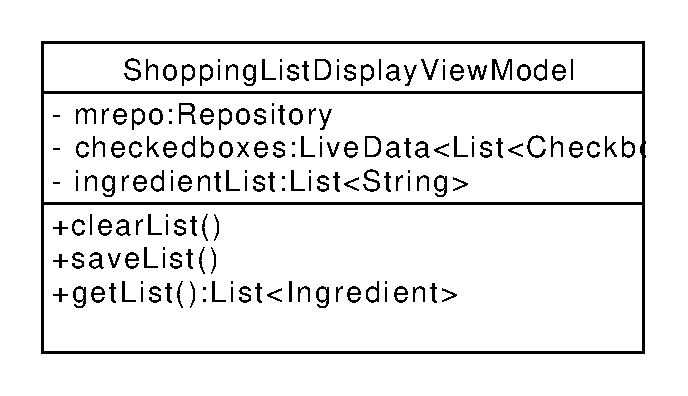
\includegraphics[width=0.7\textwidth]{pics/viewModel/Shopping_List_ViewModel.pdf}%
	\caption{ShoppingListDisplayViewModel}%
	\label{viewModel}%
\end{figure}
\begin{itemize}
	\item \textcolor{blue}{clearList()} \textcolor{cyan}{:void}
	entfernt alle Einträgte der Shoppinglist
	\item \textcolor{blue}{saveList()} \textcolor{cyan}{:void} speichert die Liste mit allen abgehakten Zuteten \textbf{F21, F24}
	\item \textcolor{blue}{getList()} \textcolor{cyan}{:List<Ingredient>} gibt die Liste an Zutaten der Liste zurück.
\end{itemize}

\subsection{FriendListViewModel}
\begin{figure}[H]
	\centering
	\includegraphics[width=0.7\textwidth]{pics/viewModel/Friend_List_ViewModel.pdf}%
	\caption{FriendListViewModel}%
	\label{viewModel}%
\end{figure}
\begin{itemize}
	\item \textcolor{blue}{loadFriends()} \textcolor{cyan}{:List<User>} lädt alle Freunde eines Nutzers und gibt diese als Liste zurück (F66)
	\item \textcolor{blue}{deleteFriend(user:User)} \textcolor{cyan}{:void} löscht einen Freund als der Freundesliste des Nutzers \textbf{F65}
	\item  \textcolor{blue}{loadRequests()} \textcolor{cyan}{:List<User>} lädt alle offenen Freundschaftsanfragen des Nutzers
	\item \textcolor{blue}{search()} \textcolor{cyan}{:void} leitet den Nutzer das UserSearchFragment weiter
	
	\item \textcolor{blue}{acceptFriendRequest(userId:String)} \textcolor{cyan}{:void} Nimmt die die Freundschaftsanfrage, ausgehen von dem Benutzer mit der userId an \textbf{F64}
	
	\item \textcolor{blue}{declineFriendRequest(userId:String)} \textcolor{cyan}{:void} Nimmt die die Freundschaftsanfrage, ausgehen von dem Benutzer mit der userId an \textbf{F64)}

\end{itemize}


\subsection{GroupMemberListViewModel}
\begin{figure}[H]
	\centering
	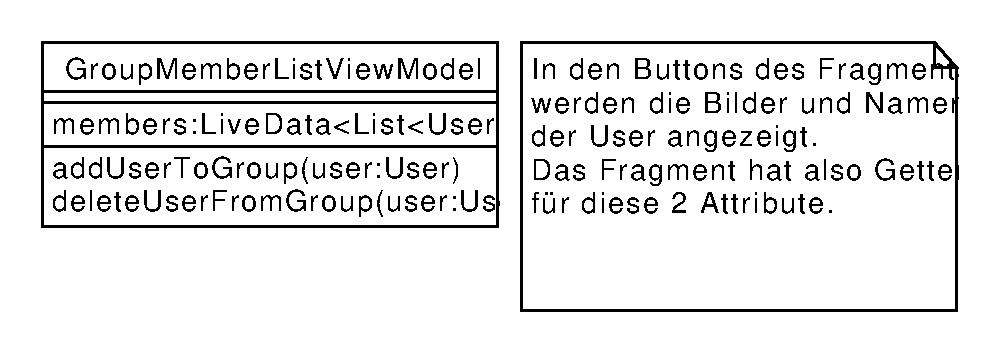
\includegraphics[width=0.7\textwidth]{pics/viewModel/Group_Member_List_ViewModel.pdf}%
	\caption{GroupMemberListViewModel}%
	\label{viewModel}%
\end{figure}
\begin{itemize}
	\item \textcolor{blue}{GroupMemberListViewModel(groupId:int)} \textcolor{cyan}{:constructor} Im Konstruktor wird übergeben, die Mitglieder welcher Gruppe übergeben werden sollen
	\item \textcolor{blue}{addUserToGroup(user:User)} \textcolor{cyan}{:void} Fügt einen Benutzer zu der Gruppe hinzu \textbf{F67}
	\item \textcolor{blue}{deleteUserFromGroup(user:User)} \textcolor{cyan}{:void} Entfernt einen Benutzer von einer Gruppe \textbf{F67}
\end{itemize}


\subsection{CreateGroupViewModel}
\begin{figure}[H]
	\centering
	\includegraphics[width=0.7\textwidth]{pics/viewModel/Create_Group_ViewModel.pdf}%
	\caption{CreateGroupViewModel}%
	\label{viewModel}%
\end{figure}
\begin{itemize}
	\item \textcolor{blue}{loadFriends()} \textcolor{cyan}{:List<User>}
	lädt alle Freunde des Nutzers und gibt diese als Liste zurück
	\item \textcolor{blue}{createGroup(memberList:List<User>)} \textcolor{cyan}{:Group} erstellt eine neue Gruppe mit allen ausgewählten Freunden. \textbf{F68}
\end{itemize}

\subsection{FriendGroupViewModel}
\begin{figure}[H]
	\centering
	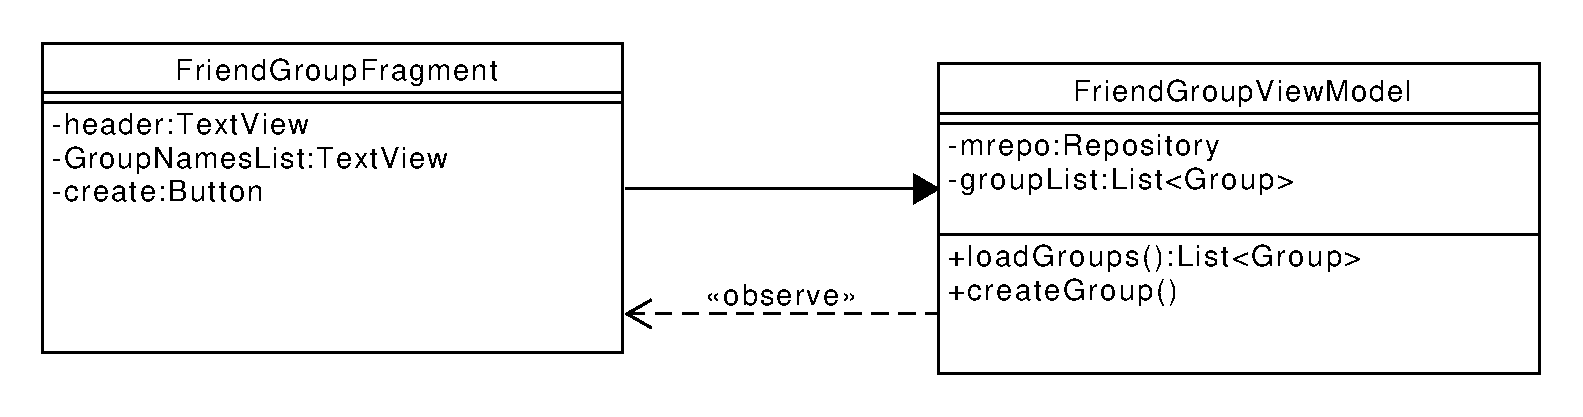
\includegraphics[width=0.7\textwidth]{pics/viewModel/Friend_Group_ViewModel.pdf}%
	\caption{FriendGroupViewModel}%
	\label{viewModel}%
\end{figure}
\begin{itemize}
	\item \textcolor{blue}{loadGroups()} \textcolor{cyan}{:List<Group>}
	lädt alle Gruppen, in den der Nutzer Mitglied ist
	\item \textcolor{blue}{createGroup()} \textcolor{cyan}{:void} leitet den Nutzer auf das createGroupFragment weiter
\end{itemize}
 

\subsection{GroupViewModel}
\begin{figure}[H]
	\centering
	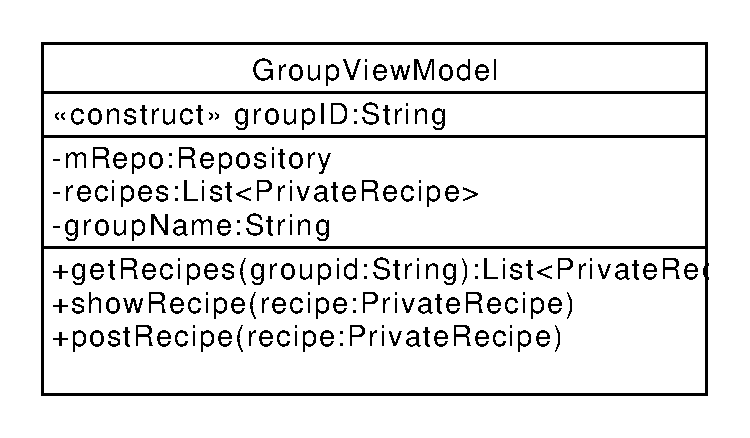
\includegraphics[width=0.7\textwidth]{pics/viewModel/Group_ViewModel.pdf}%
	\caption{GroupViewModel}%
	\label{viewModel}%
\end{figure}
\begin{itemize}
	\item \textcolor{blue}{GroupViewModel(groupId:int)} \textcolor{cyan}{:constructor} Im Konstruktor wird übergeben, um welche Gruppe es sich handelt
	\item \textcolor{blue}{getRecipes(groupid:String)} \textcolor{cyan}{:List<PrivateRecipe>}
	liefert alle privaten Rezept, die in dieser Gruppe gesendet wurden.
	
	\item \textcolor{blue}{showRecipe(recipe:PrivateRecipe)} \textcolor{cyan}{:void}
	wechselt zu dem CreateRecipeFragment
	
	\item \textcolor{blue}{postRecipe(recipe:PrivateRecipe)} \textcolor{cyan}{:void} schickt ein Rezept in die Gruppe  \textbf{F69}
\end{itemize}


\subsection{RecipeDisplayViewModel}
\begin{figure}[H]
	\centering
	\includegraphics[width=0.7\textwidth]{pics/viewModel/Recipe_Display_ViewModel.pdf}%
	\caption{RecipeDisplayViewModel}%
	\label{viewModel}%
\end{figure}
\begin{itemize}
	\item \textcolor{blue}{RecipeDisplayViewModel(recipe:PrivateRecipe)} \textcolor{cyan}{:constructor} Im Konstruktor wird übergeben, welches Rezept angezeigt werden soll \textbf{F33, F35}
	
	\item \textcolor{blue}{favorite()} \textcolor{cyan}{:void}
	falls der Nutzer angemeldet ist, favorisiert dieser das angezeigte Rezept \textbf{F18}
	
	\item \textcolor{blue}{getUser(recipe:PublicRecipe)} \textcolor{cyan}{:User}
	gibt den Ersteller eines öffentlichen Rezeptes zurück
	
	\item \textcolor{blue}{addToShoppinglist()} \textcolor{cyan}{:void}
	fügt alle Zutaten des Rezeptes mit eingestellten Mengenangaben zur Shoppinglist hinzu \textbf{F22, F23}
	
	\item \textcolor{blue}{scale()} \textcolor{cyan}{:void}
	skaliert das Rezept mit der eingegebenen Portionenzahl \textbf{F20}
	
	\item \textcolor{blue}{rate()} \textcolor{cyan}{:void}
	gibt die vom Benutzer eingegebene Bewertung ab \textbf{F34}
	
	\item \textcolor{blue}{markAsEvil()} \textcolor{cyan}{:void}
	markiert das Rezept in der Onlinedatenbank als gemeldet
	
	\item \textcolor{blue}{comment(comment:Comment)} \textcolor{cyan}{:void} Es wird in das AddEditCommentFragment gewechselt, wenn comment Null Pointer, dann wird ein Neues Kommentar erstellt, wenn nicht, dann wird dieses Kommentar bearbeitet \textbf{F36, F37}
	
\end{itemize}

\subsection{FavouriteViewModel}

\begin{figure}[H]
	\centering
	\includegraphics[width=0.7\textwidth]{pics/viewModel/Favourite_ViewModel.pdf}%
	\caption{FavouriteViewModel}%
	\label{viewModel}%
\end{figure}
\begin{itemize}
	\item \textcolor{blue}{showRecipe(recipe:PublicRecipe)} \textcolor{cyan}{:void}
	wechselt in das RecipeDisplayFragment mit dem eingegebenen Rezept
	
	\item \textcolor{blue}{removeFromFav(recipe:PublicRecipe)} \textcolor{cyan}{:void}
	löscht das Rezept von der Favoritenliste
\end{itemize}
